% !TEX program = xelatex
% Every Thing Computer at TIAT — one-sheet plan for the three plinths.
% Modelled on papers/new-urls-fall-2026/new-urls-fall-2026.tex.
\documentclass[10pt]{article}
\usepackage[paperwidth=8.5in,paperheight=11in,top=0.38in,bottom=0.36in,left=0.55in,right=0.55in]{geometry}
\usepackage{fontspec}
\usepackage{xcolor}
\usepackage{graphicx}
\usepackage{tabularx}
\usepackage{array}
\usepackage{ragged2e}
\usepackage{microtype}
\usepackage{tikz}
\usetikzlibrary{positioning,arrows.meta,calc}
\usepackage{hyperref}
\hypersetup{colorlinks=true,urlcolor=acblue,linkcolor=acdark,pdftitle={Every Thing Computer at TIAT: the three plinths}}

\setmainfont{lmsans10-regular.otf}[
  BoldFont=lmsans10-bold.otf,
  ItalicFont=lmsans10-oblique.otf,
  BoldItalicFont=lmsans10-boldoblique.otf,
]
\setmonofont{lmmonolt10-regular.otf}[Scale=0.92,
  BoldFont=lmmonolt10-bold.otf,
  ItalicFont=lmmonolt10-oblique.otf,
]
\newfontfamily\acbold{ywft-processing-bold}[Path=../../system/public/type/webfonts/,Extension=.ttf]
\newcommand{\dsep}{{\normalfont\;\textperiodcentered\;}}

\definecolor{acpink}{HTML}{B44887}
\definecolor{acblue}{HTML}{1559A6}
\definecolor{acdark}{HTML}{312B38}
\definecolor{acgray}{HTML}{66636A}
\definecolor{acpale}{HTML}{F4F1F5}
\definecolor{acrule}{HTML}{DCD6DF}
\definecolor{acgreen}{HTML}{2D7650}
\definecolor{acorange}{HTML}{A85D24}
\definecolor{neo}{HTML}{8FD13F}
\definecolor{blueberry}{HTML}{5A57D3}
\definecolor{frisbee}{HTML}{F2A7B9}
\newcommand{\acdot}{{\color{acpink}.}}
\newcommand{\ac}{Aesthetic{\acdot}Computer}

\pagestyle{empty}
\setlength{\parindent}{0pt}
\setlength{\parskip}{0pt}
\hyphenpenalty=10000\exhyphenpenalty=10000

\newcommand{\kicker}[1]{{\ttfamily\fontsize{8pt}{9.5pt}\selectfont\color{acpink}\textls[80]{#1}\par}}
\newcommand{\row}[2]{%
  \par\nointerlineskip{\color{acrule}\hrule height 0.5pt}\vspace{0.22em}%
  {\ttfamily\bfseries\fontsize{8.6pt}{10pt}\selectfont\color{acdark}#1}\par\vspace{0.08em}%
  {\fontsize{8.8pt}{10.6pt}\selectfont\color{acdark}\RaggedRight#2\par}\vspace{0.22em}}
\newcommand{\pill}[2]{{\fontsize{6.2pt}{7pt}\selectfont\colorbox{#1!12}{\textcolor{#1}{\bfseries\textls[60]{#2}}}}}
\newcommand{\hd}[1]{{\ttfamily\bfseries\fontsize{8.6pt}{10pt}\selectfont\color{acdark}#1}}

\begin{document}

% ═══════════════════════════════════════ masthead
\kicker{AESTHETIC.COMPUTER\dsep TIAT\dsep 151 POWELL ST\dsep SAN FRANCISCO}
\vspace{0.25em}
{\acbold\fontsize{34pt}{34pt}\selectfont\color{acdark}Three plinths\ \ {\color{acpink}two acts}\par}
\vspace{0.45em}
{\fontsize{11.2pt}{14pt}\selectfont\color{acdark}\RaggedRight
At the opening of \emph{Every Thing Computer} the MacNeoPolitan Trio sings on the three plinths. For the finale the three AC OS laptops under them are opened and booted, one by one, and they hold the plinths for the run.\par}
\vspace{0.3em}
{\fontsize{8.2pt}{10pt}\selectfont\color{acgray}\href{https://prompt.ac/@jeffrey}{\color{acblue}\textbf{@jeffrey}}\ \textperiodcentered\ \ac{}\ \textperiodcentered\ 2026-10-20, from Ash Herr's emails and texts\par}
\vspace{0.3em}
{\color{acdark}\rule{\linewidth}{2.5pt}}\par
\vspace{0.35em}

% ═══════════════════════════════════════ act one diagram
\kicker{ACT ONE\dsep THURSDAY 22 OCTOBER\dsep THE TRIO ON THE PLINTHS}
\vspace{0.3em}
\begin{center}\vspace{-0.3em}
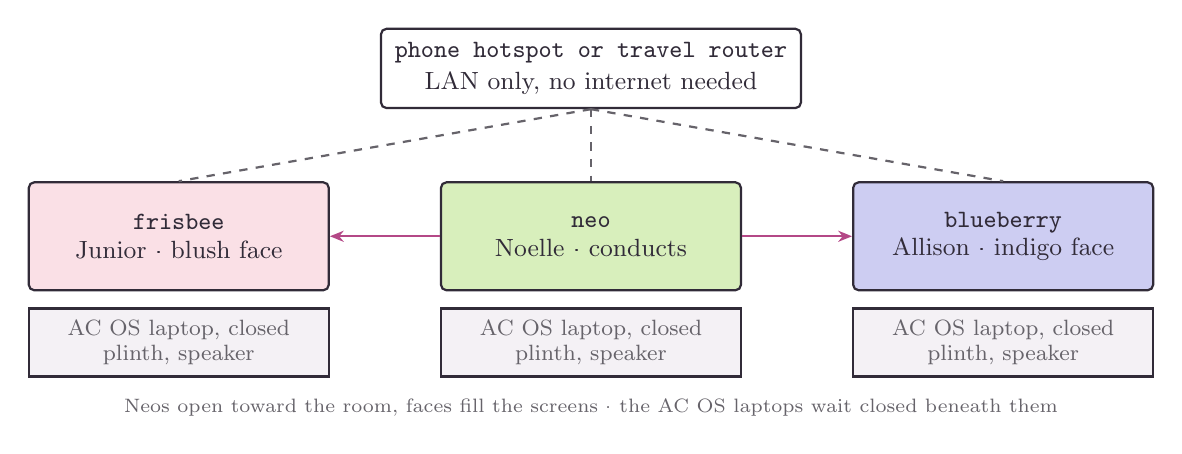
\begin{tikzpicture}[
  plinth/.style={draw=acdark, line width=0.8pt, fill=acpale, minimum width=1.5in, minimum height=0.34in, align=center, inner sep=4pt, font=\fontsize{7.6pt}{9pt}\selectfont\color{acgray}},
  lap/.style={draw=acdark, line width=0.8pt, rounded corners=2pt, minimum width=1.5in, minimum height=0.54in, align=center, inner sep=5pt, font=\fontsize{8.6pt}{10.4pt}\selectfont\color{acdark}},
  net/.style={draw=acdark, line width=0.8pt, rounded corners=2pt, fill=white, minimum width=1.9in, minimum height=0.36in, align=center, inner sep=5pt, font=\fontsize{8.6pt}{10.4pt}\selectfont\color{acdark}},
  arr/.style={-{Stealth[length=5pt,width=4pt]}, line width=0.8pt, draw=acpink},
  lan/.style={line width=0.8pt, draw=acgray, dashed}
]
\node[net] (hub) {\hd{phone hotspot or travel router}\\[1pt]LAN only, no internet needed};
\node[lap, fill=frisbee!35, below left=0.36in and 0.25in of hub] (f) {\hd{frisbee}\\Junior\ \textperiodcentered\ blush face};
\node[lap, fill=neo!35, below=0.36in of hub] (n) {\hd{neo}\\Noelle\ \textperiodcentered\ conducts};
\node[lap, fill=blueberry!30, below right=0.36in and 0.25in of hub] (b) {\hd{blueberry}\\Allison\ \textperiodcentered\ indigo face};
\node[plinth, below=0.08in of f] (pf) {AC OS laptop, closed\\plinth, speaker};
\node[plinth, below=0.08in of n] (pn) {AC OS laptop, closed\\plinth, speaker};
\node[plinth, below=0.08in of b] (pb) {AC OS laptop, closed\\plinth, speaker};
\draw[lan] (hub.south) -- (f.north);
\draw[lan] (hub.south) -- (n.north);
\draw[lan] (hub.south) -- (b.north);
\draw[arr] (n.west) -- (f.east);
\draw[arr] (n.east) -- (b.west);
\node[font=\fontsize{7.4pt}{8.5pt}\selectfont\color{acgray}, anchor=north] at ($(pn.south)+(0,-0.06in)$) {Neos open toward the room, faces fill the screens\ \textperiodcentered\ the AC OS laptops wait closed beneath them};
\end{tikzpicture}
\end{center}
\vspace{0.15em}

\begin{minipage}[t]{0.47\linewidth}\vspace{0pt}
\kicker{THE SET, ABOUT FIVE MINUTES}
\vspace{0.2em}
\row{Birth\hfill 83 s}{Canon of entries: neo alone, blueberry 48 beats in, frisbee on its own birthday beat. Each sings the date and minute it was born.}
\row{Service\hfill 53 s}{One pulse per battery cycle. Frisbee falls silent first, blueberry at 42 s, neo plays on alone.}
\row{Chorus\hfill 22 s}{One autobiography line each, then all three: \emph{Some things run in the family.}}
\row{Vocalise\hfill closer}{Row Row Row Your Boat needs the whole CultureHub rig. The ballad runs over six minutes.}
\row{Finale}{Close each Neo. Open and boot the AC OS laptop beneath it, left to right. Then the room tries notepat, aesel, or whatever they type.}
\end{minipage}\hfill{\color{acrule}\vrule width 1pt}\hfill
\begin{minipage}[t]{0.47\linewidth}\vspace{0pt}
\kicker{THE DAY}
\vspace{0.2em}
\row{Wed 21 Oct\hfill 12 to 8 pm}{Normal install window. Open to you if you arrive a day early. Not yet confirmed with Ash.}
\row{Thu 22 Oct\hfill noon}{Agreed install slot. Plinths set, network up, one dry run.}
\row{Thu\hfill by 5 pm}{Artists arrive. Bites and drinks.}
\row{Thu\hfill 6 to 7 pm}{Private preview. Press, patrons, select SF art people. Two-minute talk, or the machines sing it.}
\row{Thu\hfill 7 to 9 pm}{Public opening. Invite everyone. The set plays here.}
\row{Thu\hfill after the set}{The AC OS laptops are already up. The Neos go home.}
\end{minipage}\par

\vspace{0.4em}
{\color{acdark}\rule{\linewidth}{2.5pt}}\par
\vspace{0.38em}

% ═══════════════════════════════════════ act two diagram
\kicker{ACT TWO\dsep FROM THE FINALE THROUGH THE RUN\dsep THREE AC OS LAPTOPS, ONE CHANNEL}
\vspace{0.3em}
\begin{center}\vspace{-0.3em}
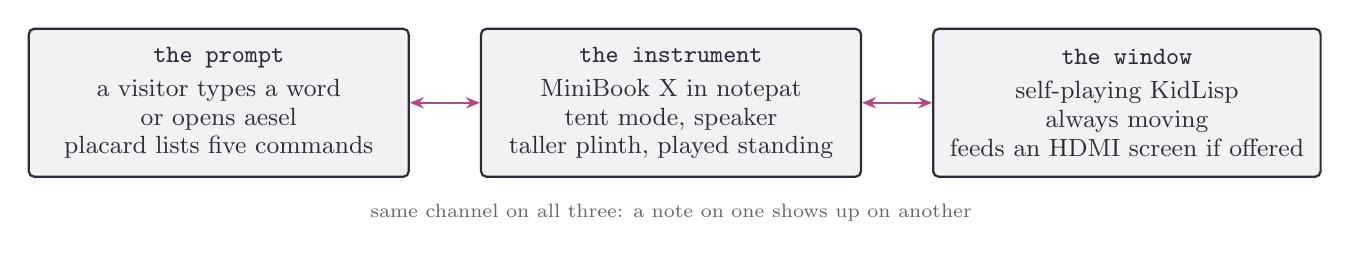
\begin{tikzpicture}[
  lap/.style={draw=acdark, line width=0.8pt, rounded corners=2pt, fill=acpale, minimum width=1.9in, minimum height=0.74in, align=center, inner sep=6pt, font=\fontsize{8.6pt}{10.4pt}\selectfont\color{acdark}},
  arr/.style={{Stealth[length=5pt,width=4pt]}-{Stealth[length=5pt,width=4pt]}, line width=0.8pt, draw=acpink}
]
\node[lap] (p) {\hd{the prompt}\\[2pt]a visitor types a word\\or opens aesel\\placard lists five commands};
\node[lap, right=0.35in of p] (i) {\hd{the instrument}\\[2pt]MiniBook X in notepat\\tent mode, speaker\\taller plinth, played standing};
\node[lap, right=0.35in of i] (w) {\hd{the window}\\[2pt]self-playing KidLisp\\always moving\\feeds an HDMI screen if offered};
\draw[arr] (p.east) -- (i.west);
\draw[arr] (i.east) -- (w.west);
\node[font=\fontsize{7.4pt}{8.5pt}\selectfont\color{acgray}, anchor=north] at ($(i.south)+(0,-0.08in)$) {same channel on all three: a note on one shows up on another};
\end{tikzpicture}
\end{center}
\vspace{0.15em}
{\fontsize{8.6pt}{10.6pt}\selectfont\color{acdark}\RaggedRight
Closing date unpublished. The previous show ran three weeks (25 September to 17 October). Gallery hours Thursday and Friday 2 to 6 pm and Saturday. These three machines are the ones that can stay, and the ones for sale.\par}

\vspace{0.4em}
{\color{acdark}\rule{\linewidth}{2.5pt}}\par
\vspace{0.35em}

% ═══════════════════════════════════════ footer: before thursday
\kicker{BEFORE THURSDAY}
\vspace{0.3em}
\begin{minipage}[t]{0.31\linewidth}\vspace{0pt}
\row{blueberry}{Offline since last night. Wake it, ship the current Menu Band build from neo, confirm all three match. Frisbee cannot compile Swift.}
\row{Wednesday morning}{One full three-body run at home with a clean stop, tap-verified. Birth, Service and Chorus ran clean in the simulator 20 Oct.}
\end{minipage}\hfill
\begin{minipage}[t]{0.31\linewidth}\vspace{0pt}
\row{The voice cast}{Noelle and Allison lose about one word in five to Whisper. Samantha and Moira lose one in twenty. In a loud room the words are the piece.}
\row{Pack}{Three Neos, three AC OS laptops, three powered speakers, travel router, power strips, HDMI cable.}
\end{minipage}\hfill
\begin{minipage}[t]{0.31\linewidth}\vspace{0pt}
\row{Text Ash}{Wednesday or Thursday only. A performance at the opening, not a demo. Three plinths in a row, standing height. Power at each.}
\row{Placard form}{Due Monday, asked again Tuesday. Not confirmed sent. \pill{acorange}{CHECK}}
\end{minipage}\par
\end{document}
